\documentclass[a4paper,11pt]{article}
%\documentclass[a4paper,9pt,landscape]{article}
\usepackage[english]{babel}
%\usepackage[utf8]{inputenc}
\usepackage{graphicx}
\usepackage{fullpage}
\usepackage{amsmath}
\usepackage{pdfpages}
\usepackage{listings}
\usepackage{color}
\usepackage{multicol}
\usepackage{fancyhdr}
\usepackage[top=1.5cm, bottom=4cm, left=2.5cm, right=2.5cm]{geometry}
\usepackage{hyperref}
\usepackage{verbatim}
\setlength{\voffset}{-9pt}
%\setlength{\hoffset}{-1in}
%\setlength{\marginparsep}{0.5cm}


\setlength{\parindent}{1cm}
%\setlength{\parskip}{-0.1cm}
%\setlength{\columnseprule}{0.4pt}
\setlength{\footskip}{0.5cm}
\setlength{\headheight}{15pt}
\setlength{\headsep}{2cm}

\fancypagestyle{tcr}{%
  \fancyhf{} %clear all headers and footers fields
  \fancyhead[R]{\thepage}
  \fancyhead[L]{\textbf{Lab No 1 TDDC78}}
  \renewcommand{\headrulewidth}{0.4pt}
}

\definecolor{dkgreen}{rgb}{0,0.6,0}
\definecolor{gray}{rgb}{0.5,0.5,0.5}
\definecolor{mauve}{rgb}{0.58,0,0.82}
\lstset{
  title=\lstname,
  frame=t,
  %aboveskip=-0.5cm, 
  %belowskip=0pt,
  basicstyle=\footnotesize\ttfamily,
  keywordstyle=\color{blue},          % keyword style
  commentstyle=\color{dkgreen},       % comment style
  stringstyle=\color{mauve},         % string literal style
  showstringspaces=false,         % underline spaces within strings
  tabsize=2,
  language=C,
  title=\caption,
  %xleftmargin=-1cm
}


\begin{document}
%% title stuff
\title{Lab No 1 TDDC78}
\author{Linus Mellberg (linme560) \and Oskar Aagaard (oskaa489)}
\date{\today}
\maketitle
\pagebreak
%\setcounter{page}{1}
%\begin{multicols}{2}
\thispagestyle{tcr}
\pagestyle{tcr}
%\tableofcontents

\section{Averaging filter}
The averaging filter works by convoluting the input image with a gaussian filter kernel.
This will do a weighted average on the pixel and the pixels surrounding it.
Since the gaussian kernel is symmetric the the calculation can be simplified, this makes the problem linear in the radius of the kernel.
\subsection{Description of the program}
The program uses the MPI framework for communication between the processes.
Parallelization is done by splitting the picture into equal regions along the y-axis.
Each process then apply the filter on the region that is given to it. 
Since the filter does averaging on the neighbouring pixels each process needs more data than the pixels which it filters.
This makes it neccesary to send more data to each process than the data that belongs to the region which it filters.

The process with rank 0 reads the image from disk.
When this is done it broadcast the dimension of the picture.
Every process then calculates how the picture is divided into regions and shared between the processes.
When this is done the rank 0 process send the data to the processes, each process gets all data needed to do its own filtering.
As soon as a process has recieved its data it will start applying the filter to it.
The rank 0 process also gets a region of the image and start processing as soon as possible.
When the processes are done with the filtering a \emph{MPI\_Gatherv} operation is performed to collect all the data at the rank 0 process.
This process then writes the filtered image to disk.

At first the nonblocking send was used to distribute data to the processes.
When the program was analyzed with traceanalyzer it was discovered that this is not a good thing to do.
The nonblocking send does not send the data immediately.
It seems that what is done is put the data into a buffer and send this when another MPI call is waiting to complete.
The result of this behavoiur is that the root process completes its own filtering before sending any data to the other processes.
This makes all the other processes idle while the root process filter the data given to it, this effectively doubles the execution time of the program.
When using the blocking send operation all data is sent before any filtering and the non-root processes are only idle when data is read and written to disk.

\subsection{Result and graphs}

If a small filter kernel is used the read and write operations becomes a large part of the execution time of the program.
A filter kernel with radius 10 run on 8 cores uses more time for reading the image from disk than to do the filtering.
This is a sequencial operation that might be possibly to optimize, but this is left out of this report.
This has made us ignore the time used for reading and writing to disk from of the execution time calculations used below.
The send operations that distribute data among the processes is still in the calculations as these are an important part of any parallel program.
The traceanlyzer tool produced the chart in figure \ref{trace} the chart is from a run on \emph{im4.ppm} with 8 cores and a filter kernel radius of 10.
Apart from the disk read/write the the load balancing seems good and the send operations are a small part of the total execution time of the program.

The execution times of this program when changing problemsize and the number of cores are more or less as expected.
The execution time is proportional to the radius of the applied filter kernel and the number of pixels in the image.
It is inversely proportional to the number of processes.
This is at least true when the size of the filter kernel is larger than 10.
When the radius is small the operations that sends and recieve data between the different processes becomes more noticeable.
This might be because the complexity of the filter operation will start to become small in comparision to the complexity of shuffling data.
There might also be cache effects or timing issues because of process initialization when the total excecution time is very low.

In figure \ref{32_cores_runtime} the execution time hardly increases at all when increasing the radius on image 1.
The filtering complexity for this image gets 100 times larger when increasing the radius 100 times, but the execution time is more or less constant.
It is such a small part of the total execution time of the program.
The size of the 3 smallest images don't influence the runt time when the radius is small either.
There seems to be about 0.03 seconds here that is wasted on starting all the processes.

In figure \ref{im4} we can see how the program performs on the largest image.
The execution time is proportional to the radius of the filter kernel.
One can also see the execution time is inversely proportional to the numbers of cores.
Figure \ref{complexity} shows how execution time changes when both the problem size and the number of cores are changed.
Each picture of the pictures 1, 2 and 3 are roughly twice as as large as the previous in terms of number of pixels.
In the plot \emph{im3.ppm} is run with twice the number of cores as \emph{im2.ppm} which is run with twice as many cores as \emph{im1.ppm}.
This should mean that each line in the plot should correspond to roughly the same computational complexity.
In the plot the lines are roughly equal as it should be.
If the problem size is larger more cores can be used to solve it in the same amount of time.

The number of floating points operations per second was also estimated.
This number should ideally be the same for all problem sizes on a fixed number of cores, it should also be proportional to the number of cores.
This is not true for small problem sizes.
When the total excecution time of the program is below about 0.03 seconds it seems to be uncorrelated with the problem size.
The reason for this might be various cache effects or initialization times for the different processes.
For the bigger problem sizes the MFLOP count converges to about 1800 MFLOP per process.

\begin{figure}[!h]
  \caption{Traceanalyzer chart for im4.ppm on 8 cores with radius 10.}
  \label{trace}
  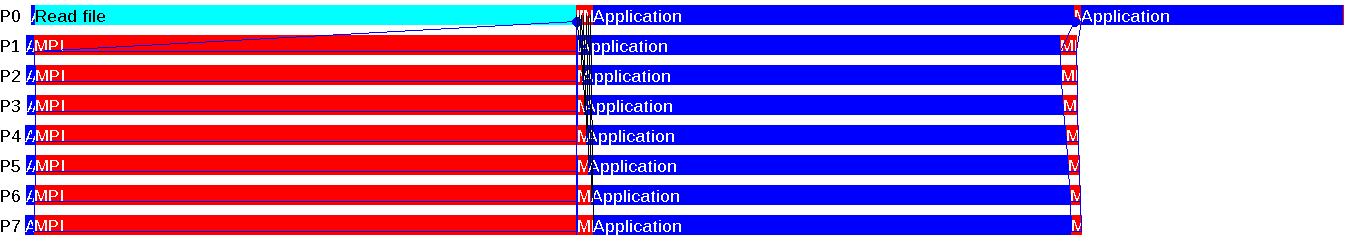
\includegraphics[width=500pt]{../plots/tracechart_r10_im4_8cores.png}
\end{figure}
\begin{figure}[!h]
  \caption{Run times related to radius on 32 cores for the different images.}
  \label{32_cores_runtime}
  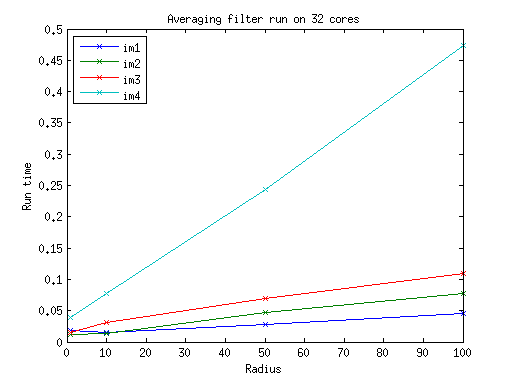
\includegraphics[scale=0.9]{../plots/32_cores_runtime_radius.png}
\end{figure}
\begin{figure}[!h]
  \caption{Run times for different numbers of cores on im4.ppm.}
  \label{im4}
  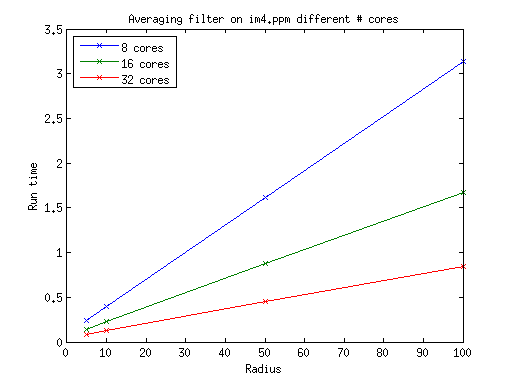
\includegraphics[scale=0.9]{../plots/im4_runtime_radius.png}
\end{figure}
\begin{figure}[!h]
  \caption{Run times related to radius when increasing image size and number of cores.}
  \label{complexity}
  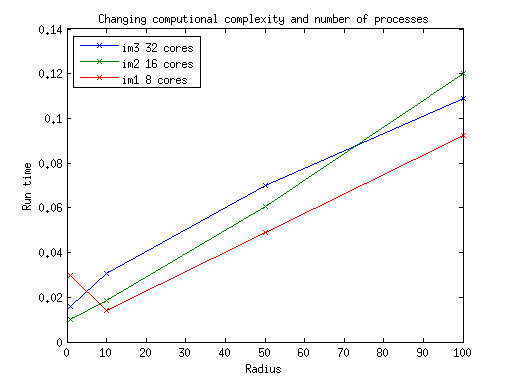
\includegraphics[scale=0.9]{../plots/compexity_and_no_processes.png}
\end{figure}

\clearpage

\section{Thresholding filter}
The thresholding filter turns a coloured image into a black and white image. A pixel in the filtered image is black if its colour intensity is lower than a threshold, otherwise white. The colour intensity is calculated by summing the RGB values of a pixel. The threshold is determined by the average colour intensity of all the pixels.
\subsection{Description of the program}
The first step is determining the average pixel intensity by adding the RGB values of each pixel in the image together and dividing by the total number of pixels. The program then looks at the RGB sum for each pixel in turn and determines if the corresponding pixel of the output image should be black or white by whether it's greater or lower than the average.

\paragraph\noindent\textbf{Overview of the linear program}
\begin{itemize}
\renewcommand{\labelitemi}{$\bullet$}
\item Load image from disk
\item Calculate average RGB sum
\item Calculate output image
\item Write image to disk
\end{itemize}

Because there is no dependency between pixels during either of the two calculations the work can easily be divided between an arbitrary amount of processors by giving them an as equal share as possible and with no locality concerns regarding reducing communication. 

The program calculates the work share of each processor and then distributes the splitted source image by using the MPI\_Scatter command. The processors then calculate the RGB sum of their share and the total sum is then calculated and redistributed for the second calculation by using the MPI\_Allreduce command.

\paragraph\noindent\textbf{Overview of the parallel program}

\begin{itemize}
\renewcommand{\labelitemi}{$\bullet$}
\item Load image from disk on root processor
\item Calculate work shares
\item Use MPI\_Scatter to distribute parts of the image
\item Calculate average RGB sum in parallel
\item Sum the results and redistributed the total sum by using MPI\_Allreduce
\item Calculate output image in parallel
\item Gather the result to the root processor by using MPI\_Gather
\item Root process writes image to disk
\end{itemize}

\subsection{Result and graphs}
In figure \ref{runtime_vs_cores} we can see that the largest image scales well to 4 cores, halving the runtime, but then barely sees any decrease in runtime when increasing the amount of cores to 8 and finally sees a slight increase in runtime for more cores than that. Because the work to be done is small compared to the blur filter but the messaging is similar we expect that this program should scale less well to many cores. It appears that the work load is in fact so small that there's quickly no gain at all. This becomes more pronounced as the problem size grows smaller to the point where the smallest image never sees any gain in increasing the amount of cores past 2.

For a single core we see that increasing the problem size will linearly increase run time. The size of \emph{im2.ppm} is very slightly more than twice that of \emph{im1.ppm} and the run time is doubled. Similarily \emph{im3.ppm} is slightly less than twice the size of \emph{im2.ppm} but and has the run time doubled again. The size of \emph{im4.ppm} is about $4.7$ times that of \emph{im3.ppm} and the run time is very close to $4.7$ times that of \emph{im3.ppm}. If we try the same for 4 cores we see that it holds up between the second, third and fourth image but not so much going from the first to the second image where the communication starts taking too much time.

This observation about the graph is also corroborated by table \ref{mpixelspersecond} which shows the number of pixels in the input image divided by run time and is proportional to MFlops. The columns show that keeping the amount of cores constant will give linear increase in run time up to a point where too many cores creates too much overhead, and this point is lower for smaller problems. If we look at the rows we can see that increasing the amount of cores will solve the problem faster up to a point where there's too much overhead.

For the scaled speed up we can look at \emph{im1.ppm}, \emph{im2.ppm} and \emph{im3.ppm} which are roughly doubling in size from one image to the next. In figure \ref{runtime_vs_cores} we can compare \emph{im1.ppm} at 4 cores with \emph{im2.ppm} at 8 cores and \emph{im3.ppm} at 16 cores. Ideally the run times should then be the same for these points but because the solution is not scaling well with cores we see that the run time in the first step is doubled and then after that tripled again in the second step.

\begin{figure}[!h]
  \caption{Run times related to number of cores for the different images.}
  \label{runtime_vs_cores}
  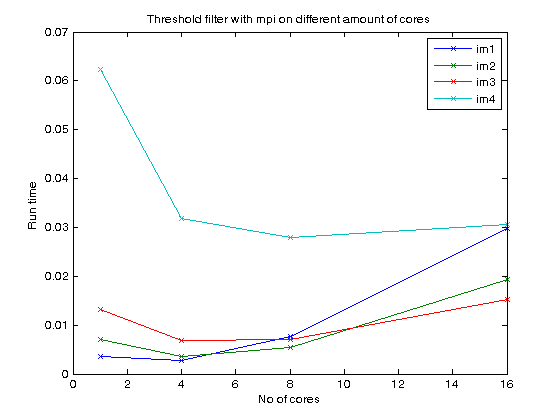
\includegraphics[scale=0.9]{../plots/runtimevscoresthres.png}
\end{figure}


\begin{table}[h!]
  \caption{$MPixels/Second$ when running with different amount of threads and on different data.}
  \label{mpixelspersecond}
  \begin{tabular}[h]{|l|l|l|l|l|l|}
    \hline
                      & 1      & 2      & 4      & 8      & 16\\
    \hline
    im1.ppm           & 135.41 & 183.31 & 184.94 & 68.89  & 21.77\\ 
    im2.ppm           & 150.01 & 209.17 & 274.71 & 201.65 & 63.15\\ 
    im3.ppm           & 146.25 & 209.72 & 274.44 & 275.62 & 138.23\\ 
    im4.ppm           & 145.07 & 212.56 & 286.41 & 332.90 & 297.42\\
    \hline
  \end{tabular}
\end{table}

\begin{comment}
\cite{fenwick}
\clearpage
\begin{thebibliography}{9}
  \bibitem{fenwick}
    Binary Indexed Trees,
    \emph{Algortihmist}.\\
    \url{http://community.topcoder.com/tc?module=Static\&d1=tutorials\&d2=binaryIndexedTrees}
  \bibitem{ppm}
    Mark Nelson,
    \emph{Arithmetic Coding + Statistical Modeling = Data Compression}, 1991.\\
    \url{http://marknelson.us/1991/02/01/arithmetic-coding-statistical-modeling-data-compression/}
  \bibitem{ppmc}
    PPM
    \url{http://www.cs.ucf.edu/courses/cap5015/ppm.pdf}

\end{thebibliography}a
\end{comment}

\clearpage
\section{Source code}
Files that are included but not listed here were downloaded from the course webpage and not modified.

\lstinputlisting[caption=mpiblur.c]{../mpiblur.c}
\clearpage
\lstinputlisting[caption=mpiblurfilter.c]{../mpiblurfilter.c}
\lstinputlisting[caption=mpiblurfilter.c]{../mpiblurfilter.h}
\clearpage
\lstinputlisting[caption=mpithreshold.c]{../mpithreshold.c}
\end{document}
